\chapter{Technische Implementierung}
\section{Elektronische Bauteile}

\subsection{Motor}\label{eb:motor}

% Tabelle
\begin{table}[!ht]
\centering
\rmfamily
\caption{Pinbelegung Motor}
\renewcommand{\arraystretch}{1.1}
\sffamily
\begin{footnotesize}
\begin{tabular}{r | l l}
\toprule
\textbf{Pin} & \textbf{Farbe}  & \textbf{Belegung}\\
\midrule
1 & Weiß & Motor +9V; PWM-Steuerung \\
2 & Schwarz & Motor -9V; PWM-Steuerung \\
3 & Rot & Ground \\
4 & Grün & +4,3V Versorgungsspannung \\
5 & Gelb & Motorencoder (Quadratur-Encoder, Kanal a) \\
6 & Blau & Motorencoder (Quadratur-Encoder, Kanal b) \\
\bottomrule
\end{tabular}
\end{footnotesize}
\label{eb:motor:tbl}
\end{table}

Die Steuerung des Motors erfogt über eine 9V Spannung. Für die Regulierung der Geschwindigkeit wird auf eine Pulsweitenmodulation zurückgeriffen. Die max. Stromstärke liegt bei 700mA für den Motor.  Die Versorgungsspannung an Pin 4 versorgt den Rotationssensor mit Strom. Mittels des Rotationssensors kann die genaue Rotationsposition des Motors bestimmt werden. Dieser Sensor kann über die Pin's 5 und 6 ausgelesen werden. Dieser Sensor wurde in diesem Projekt nicht weiter behandelt.


\subsection{Sensoren}\label{eb:sensor}


% Tabelle
\begin{table}[!ht]
\centering
\rmfamily
\caption{Pinbelegung Tastsensor}
\renewcommand{\arraystretch}{1.1}
\sffamily
\begin{footnotesize}
\begin{tabular}{r | l l}
\toprule
\textbf{Pin} & \textbf{Farbe}  & \textbf{Belegung}\\
\midrule
1 & Weiß & Trigger \\
2 & Schwarz & - \\
3 & Rot & Ground \\
4 & Grün & - \\
5 & Gelb & - \\
6 & Blau & - \\
\bottomrule
\end{tabular}
\end{footnotesize}
\label{tastsensor:tbl}
\end{table}
Der Tastsensor gehört zu den analog Sensorn vom NXT. Im Normalzustand ist der Tastsensor geöffnet (no: Normal Open). Die Leistungsaufnahme des Tastsensors ist im geöffneten zustand mit 2,2 mA sehr gering. Im geschlossenen Zustand liegt die Stromaufnahme bei 0 mA.



% Tabelle
\begin{table}[!ht]
\centering
\rmfamily
\caption{Pinbelegung Tonsensor}
\renewcommand{\arraystretch}{1.1}
\sffamily
\begin{footnotesize}
\begin{tabular}{r | l l}
\toprule
\textbf{Pin} & \textbf{Farbe}  & \textbf{Belegung}\\
\midrule
1 & Weiß & Analoges Tonsignal \\
2 & Schwarz & Ground \\
3 & Rot & Ground \\
4 & Grün & +4,3V Versorgungsspannung \\
5 & Gelb & Moduswahl dB/dBA \\
6 & Blau & Direkter Ausgang \\
\bottomrule
\end{tabular}
\end{footnotesize}
\label{tonsensor:tbl}
\end{table}
Der Tonsensor war nicht Teil dieses Projektes, jedoch wird er zur Vollständigkeit hier aufgeführt. Auch der Tonsensor ist ein Analogsensor. Dieser Senesor misst den Schalldruck zwischen 55 dB und 90 dB. Bei der Decibelskala ist zu beachten, dass es sich hier um eine Logarithmische Skalierung handelt. Somit nimmt der Mensch eine Erhöhung der Lautstärke um 10 dB als Verdopplung der Lautstärke wahr. Die Stromaufnahme des Tonsensors liegt bei 2,0 mA.
% Tabelle
\begin{table}[!ht]
\centering
\rmfamily
\caption{Pinbelegung Lichtsensor}
\renewcommand{\arraystretch}{1.1}
\sffamily
\begin{footnotesize}
\begin{tabular}{r | l l}
\toprule
\textbf{Pin} & \textbf{Farbe}  & \textbf{Belegung}\\
\midrule
1 & Weiß & Analoges Lichtsignal \\
2 & Schwarz & Ground \\
3 & Rot & Ground \\
4 & Grün & +4,3V Versorgungsspannung \\
5 & Gelb & Lichtquelle Ein/Aus \\
6 & Blau & - \\
\bottomrule
\end{tabular}
\end{footnotesize}
\label{lichtsensor:tbl}
\end{table}

Der Lichtsensor ist auch ein analoger Sensor. Über eine Lichtempfindlichen Widerstand (LDR) kann dieser Sensor die Helligkeit messen. Der Sensor hat zwei Modis. Der erste Modus ist \emph{Umgebungslicht Modus} mit einer Stromverbrauch von 2,5 mA.  Im \emph{Reflektions Modus} wird eine kleine LED aktiviert und der Stromverbrauch steigt so auf 15 mA.

% Tabelle
\begin{table}[!ht]
\centering
\rmfamily
\caption{Pinbelegung Ultraschallsensor}
\renewcommand{\arraystretch}{1.1}
\sffamily
\begin{footnotesize}
\begin{tabular}{r | l l}
\toprule
\textbf{Pin} & \textbf{Farbe}  & \textbf{Belegung}\\
\midrule
1 & Weiß & +9V Versorgungsspannung \\
2 & Schwarz & Ground \\
3 & Rot & Ground \\
4 & Grün & +4,3V Versorgungsspannung \\
5 & Gelb & I2C-Kommunikation SCL (Serial Clock) \\
6 & Blau & I2C-Kommunikation SDA (Serial Data) \\
\bottomrule
\end{tabular}
\end{footnotesize}
\label{eb:ultraschall:tbl}
\end{table}

Der ultraschall Sensor ist ein digitaler Sensor. Das bedeutet, dass das Signal mittels I2C-Bus übertragen wird. Mit diesem Sensor können Distanzen zwischen  0 cm und 255 cm gemessen werden. Es ist der einzigste Sensor der zusätzlich zu der normalen Versorgungsspannung von 4,3V noch eine 9V Versorgungsspannung benötigt.

\subsection{SN754410}\label{eb:pwm}
%Figure
\begin{wrapfigure}{r}{0.65\textwidth}
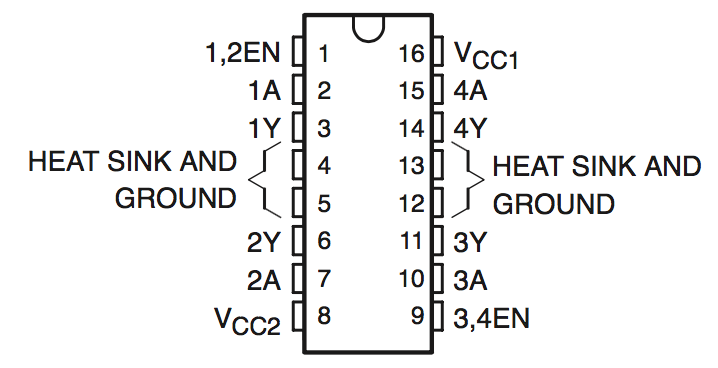
\includegraphics[width=0.9\linewidth]{bauelemente/sn754410}
\caption{SN754410}
\label{eb:fig:sn754410}
\end{wrapfigure}
Der SN754410 ermöglicht das Steuern der zwei Motoren mit einer max Stromstärke von 1 A (max Stromaufnahme eines Motors 700 mA) bei 9V. Die von uns  geschriebene Software steuert den Chip so an, dass über eine software Pulsweitenmodulation die Geschwindigkeit des Motors beliebig angepasst werden kann. Durch die Pulsweitenmodulation ist die Wärmeentwicklung sehr gering. Daher ist eine Kühlung dieses Bauteils nicht notwendig.

Über jeweils zwei GPIO-Pins kann so ein Motor gesteuert werden.

\subsection{MCP3008}\label{eb:adwandler}
%Figure
\begin{wrapfigure}{r}{0.4\textwidth}
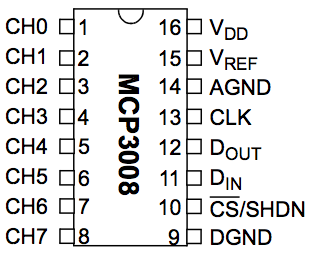
\includegraphics[width=0.9\linewidth]{bauelemente/mcp3008}
\caption{MCP3008}
\label{eb:mcp3008}
\end{wrapfigure}
Der MCP3008 ist ein Analog/Digital-Wandler (A/D-Wandler). Dieses Bauteil wird über den SPI-Bus am Raspberry Pi angeschlossen. Über den 8 Eingänge (CH0-CH7) lassen sich 8 verschiedene analoge Sensore anschließen. Der A/D-Wandler macht aus dem analogen Einganssignal einen Bitstream, der über den SPI-Bus übertragen wird.

Über vier GPIO-Pins können so 8 analoge Sensoren gesteuert werden.

\section{Elektronischer Aufbau}

\subsection{Motor}
%Figure
\begin{wrapfigure}{r}{0.65\textwidth}
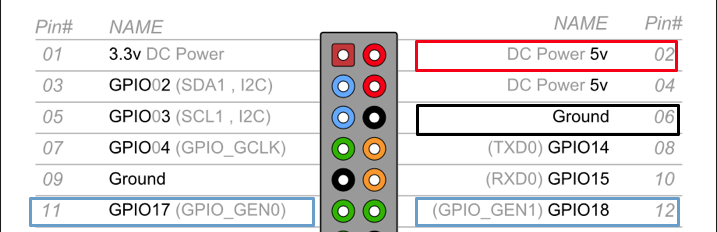
\includegraphics[width=0.9\linewidth]{schaltung/motor-pin}
\caption{GPIO Belegung Motor}
\label{ea:motor-pin}
\end{wrapfigure}
An der Pinbelegung des Motors \ref{eb:motor:tbl} ist zu erkennen, dass der Motor eine Spannung von 9V benöigt. Die Versorgungspanng von 4,3V ist für den eingebauten Controller im Motor. Pin 1 und 2 des Motors müssen mit dem in \ref{eb:pwm} beschriebenen Bauteil verbunden werden (hier Pin 14 und 10 von 754410). Die 9V Motorspannung liegt an Pin 8 (SN754410) an und kommt von einem zusätzlich 9V-Block. Übder die Pins 15 und 11 wird das Bauteil an 2 GPIO's angeschlossen. Weitere benötigte Verbindungen sind die GND, welche alle zusammen verbunden werden und die Versorgungspannung von 4,3V-5V.

Eine Vollständige Belegung der Pins für den Probeaufbau befindet sich in Abbildung \ref{ea:motor-pin}

%Figure
\begin{figure}[h]
  \centering
  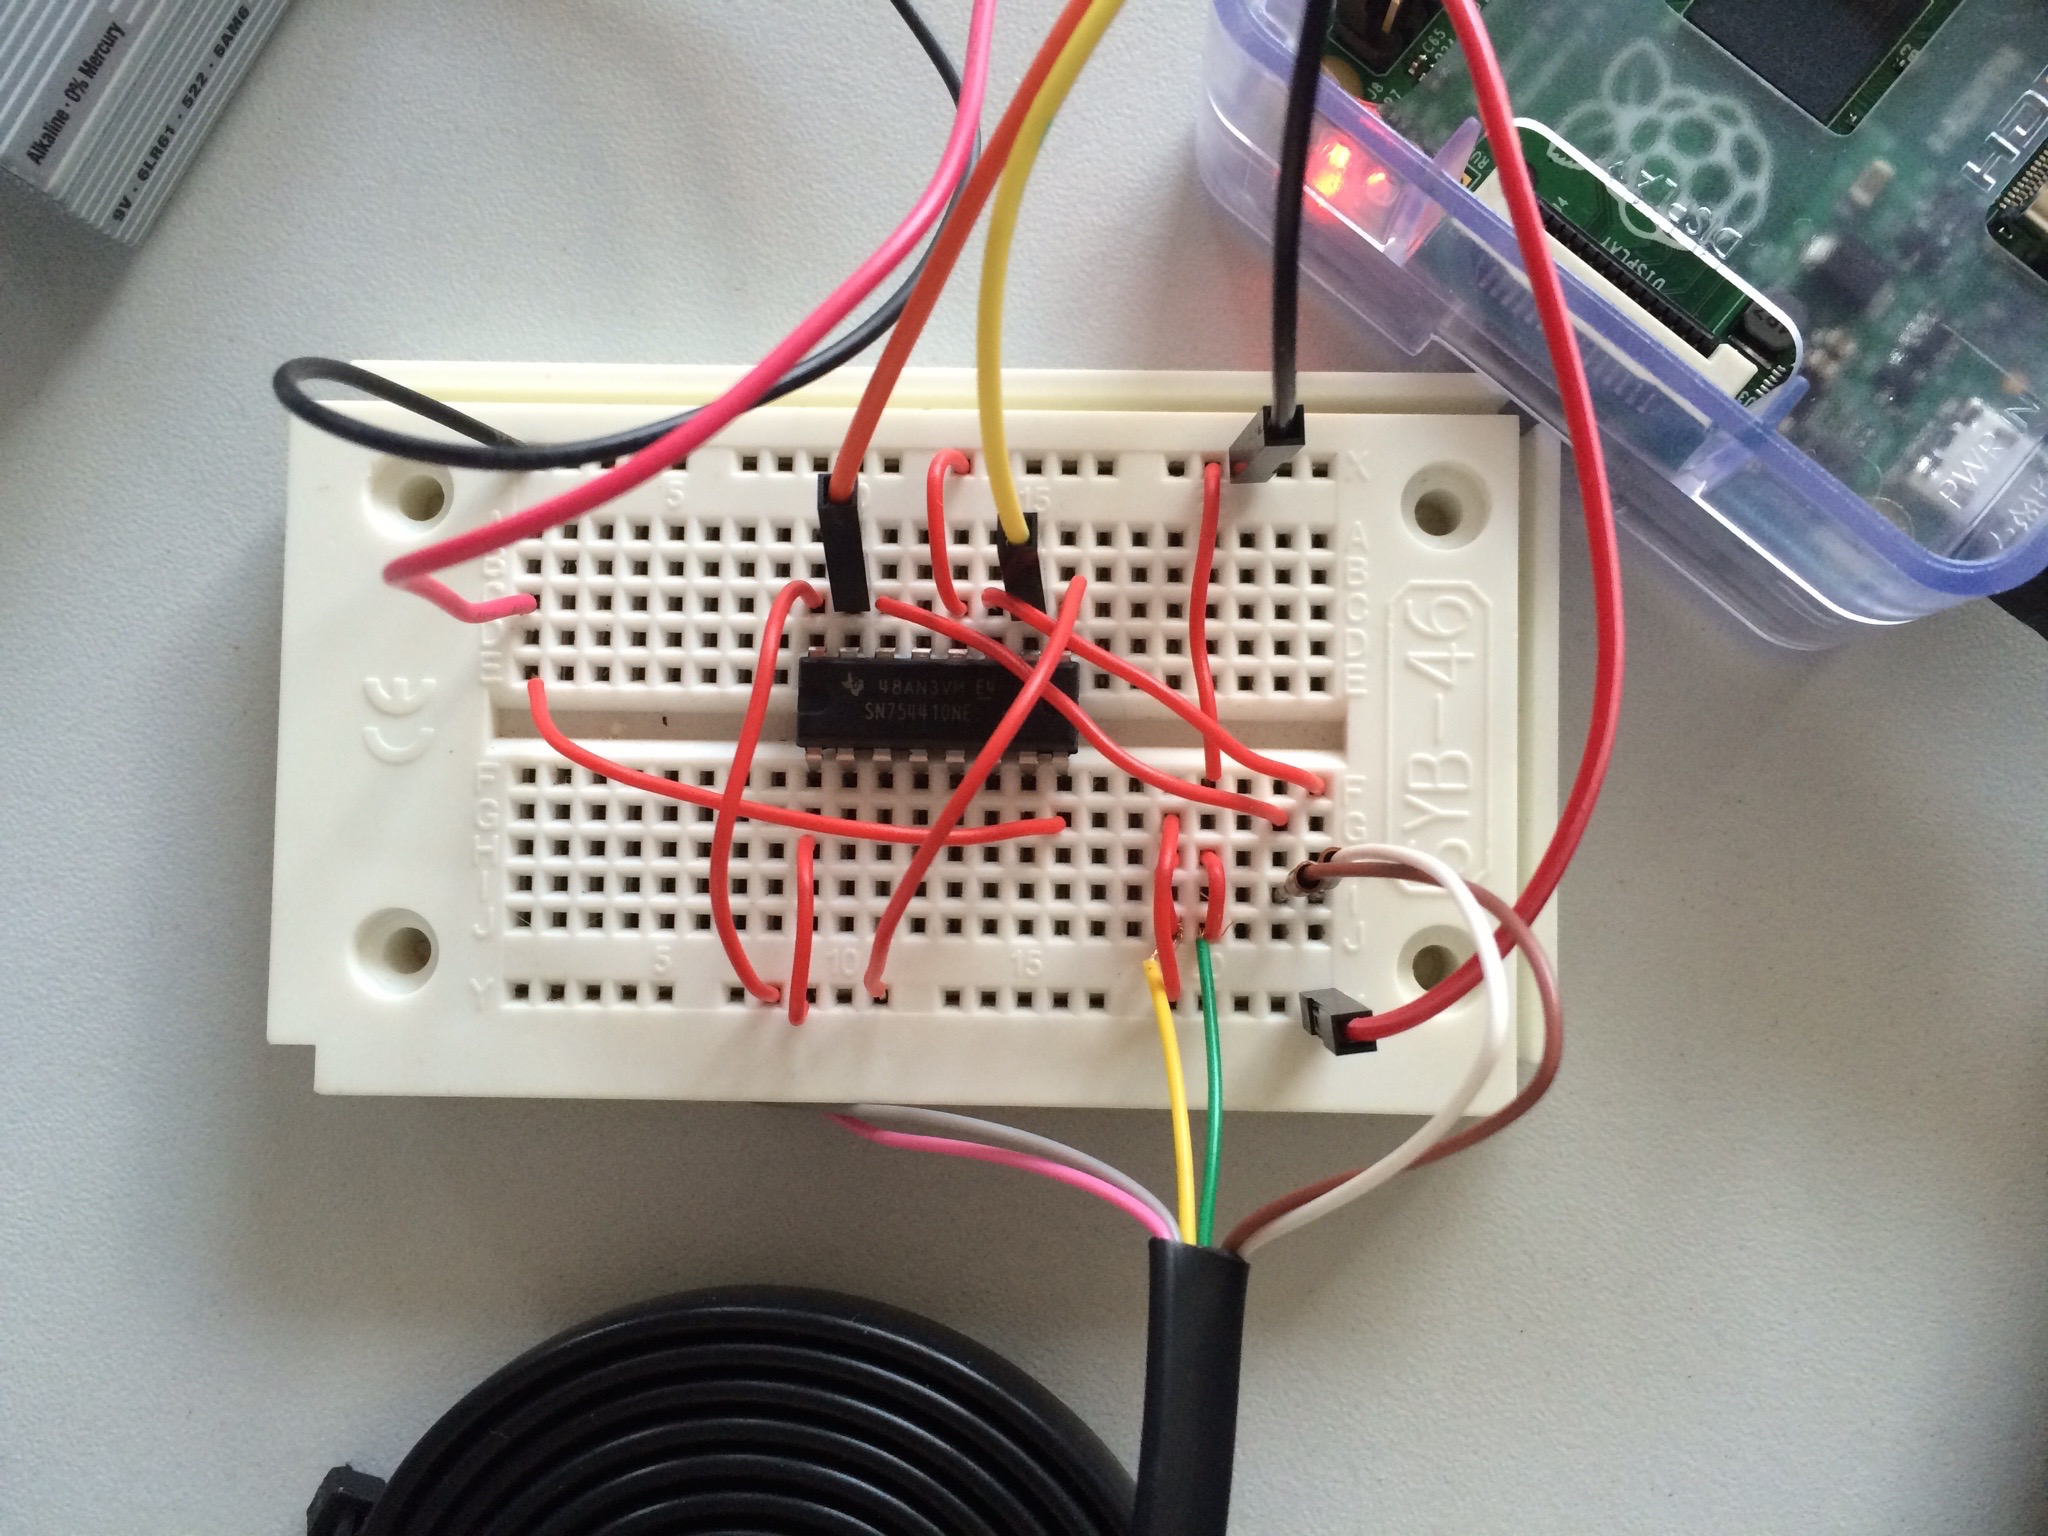
\includegraphics[width=12cm]{schaltung/motor}
  \caption{Probeaufbau Motor}
  \label{schaltung:motor}
\end{figure}

\subsection{Sensor}
%Figure
\begin{wrapfigure}{r}{0.65\textwidth}
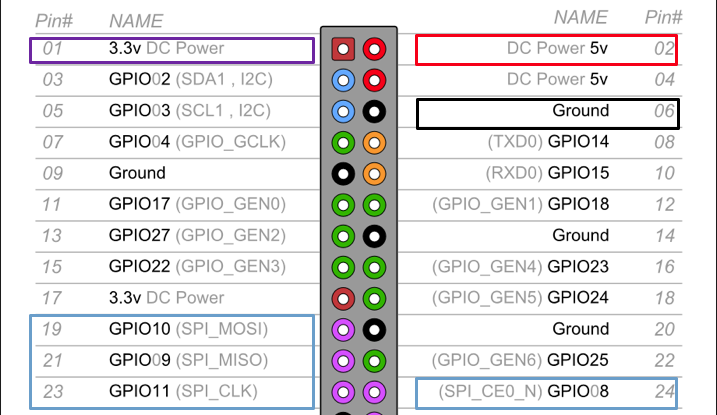
\includegraphics[width=0.9\linewidth]{schaltung/sensor-pin}
\caption{GPIO Belegung Sensor}
\label{ea:sensor-pin}
\end{wrapfigure}

Die Versorgungspannung für den MCP3008 ist hier 3,3V und die Versorgungspannung für die Sensoren sind 4,3V-5V vom Raspberry Pi. Die analogen Sensoren werden an CH0-CH7 an der A/D-Wandler über eine Spannungsteilerschaltung angeschlossen. Der Spannungteiler wird mit einem 10kOhm Widerstand realisiert (in der Probeschaltung 2* 4,7kOhm in Reihe). Mit vier Anschlusskabeln wird der A/D-Wandler über den SPI-Bur am Raspberry Pi angeschlossen. Die Erdung geschieht auch über den Raspberry. Bei dem Spezialfall \emph{Lichtsensor} wird zusätzlich für die Lichtquelle eine Versorgungsspannung benötigt. Da der PIN 5 bei dem \emph{Tastsensor} nicht belegt ist, wird standartmäßig überall der Pin 5 an 4,3V-5V angeschlossen.

%Figure
\begin{figure}[h]
  \centering
  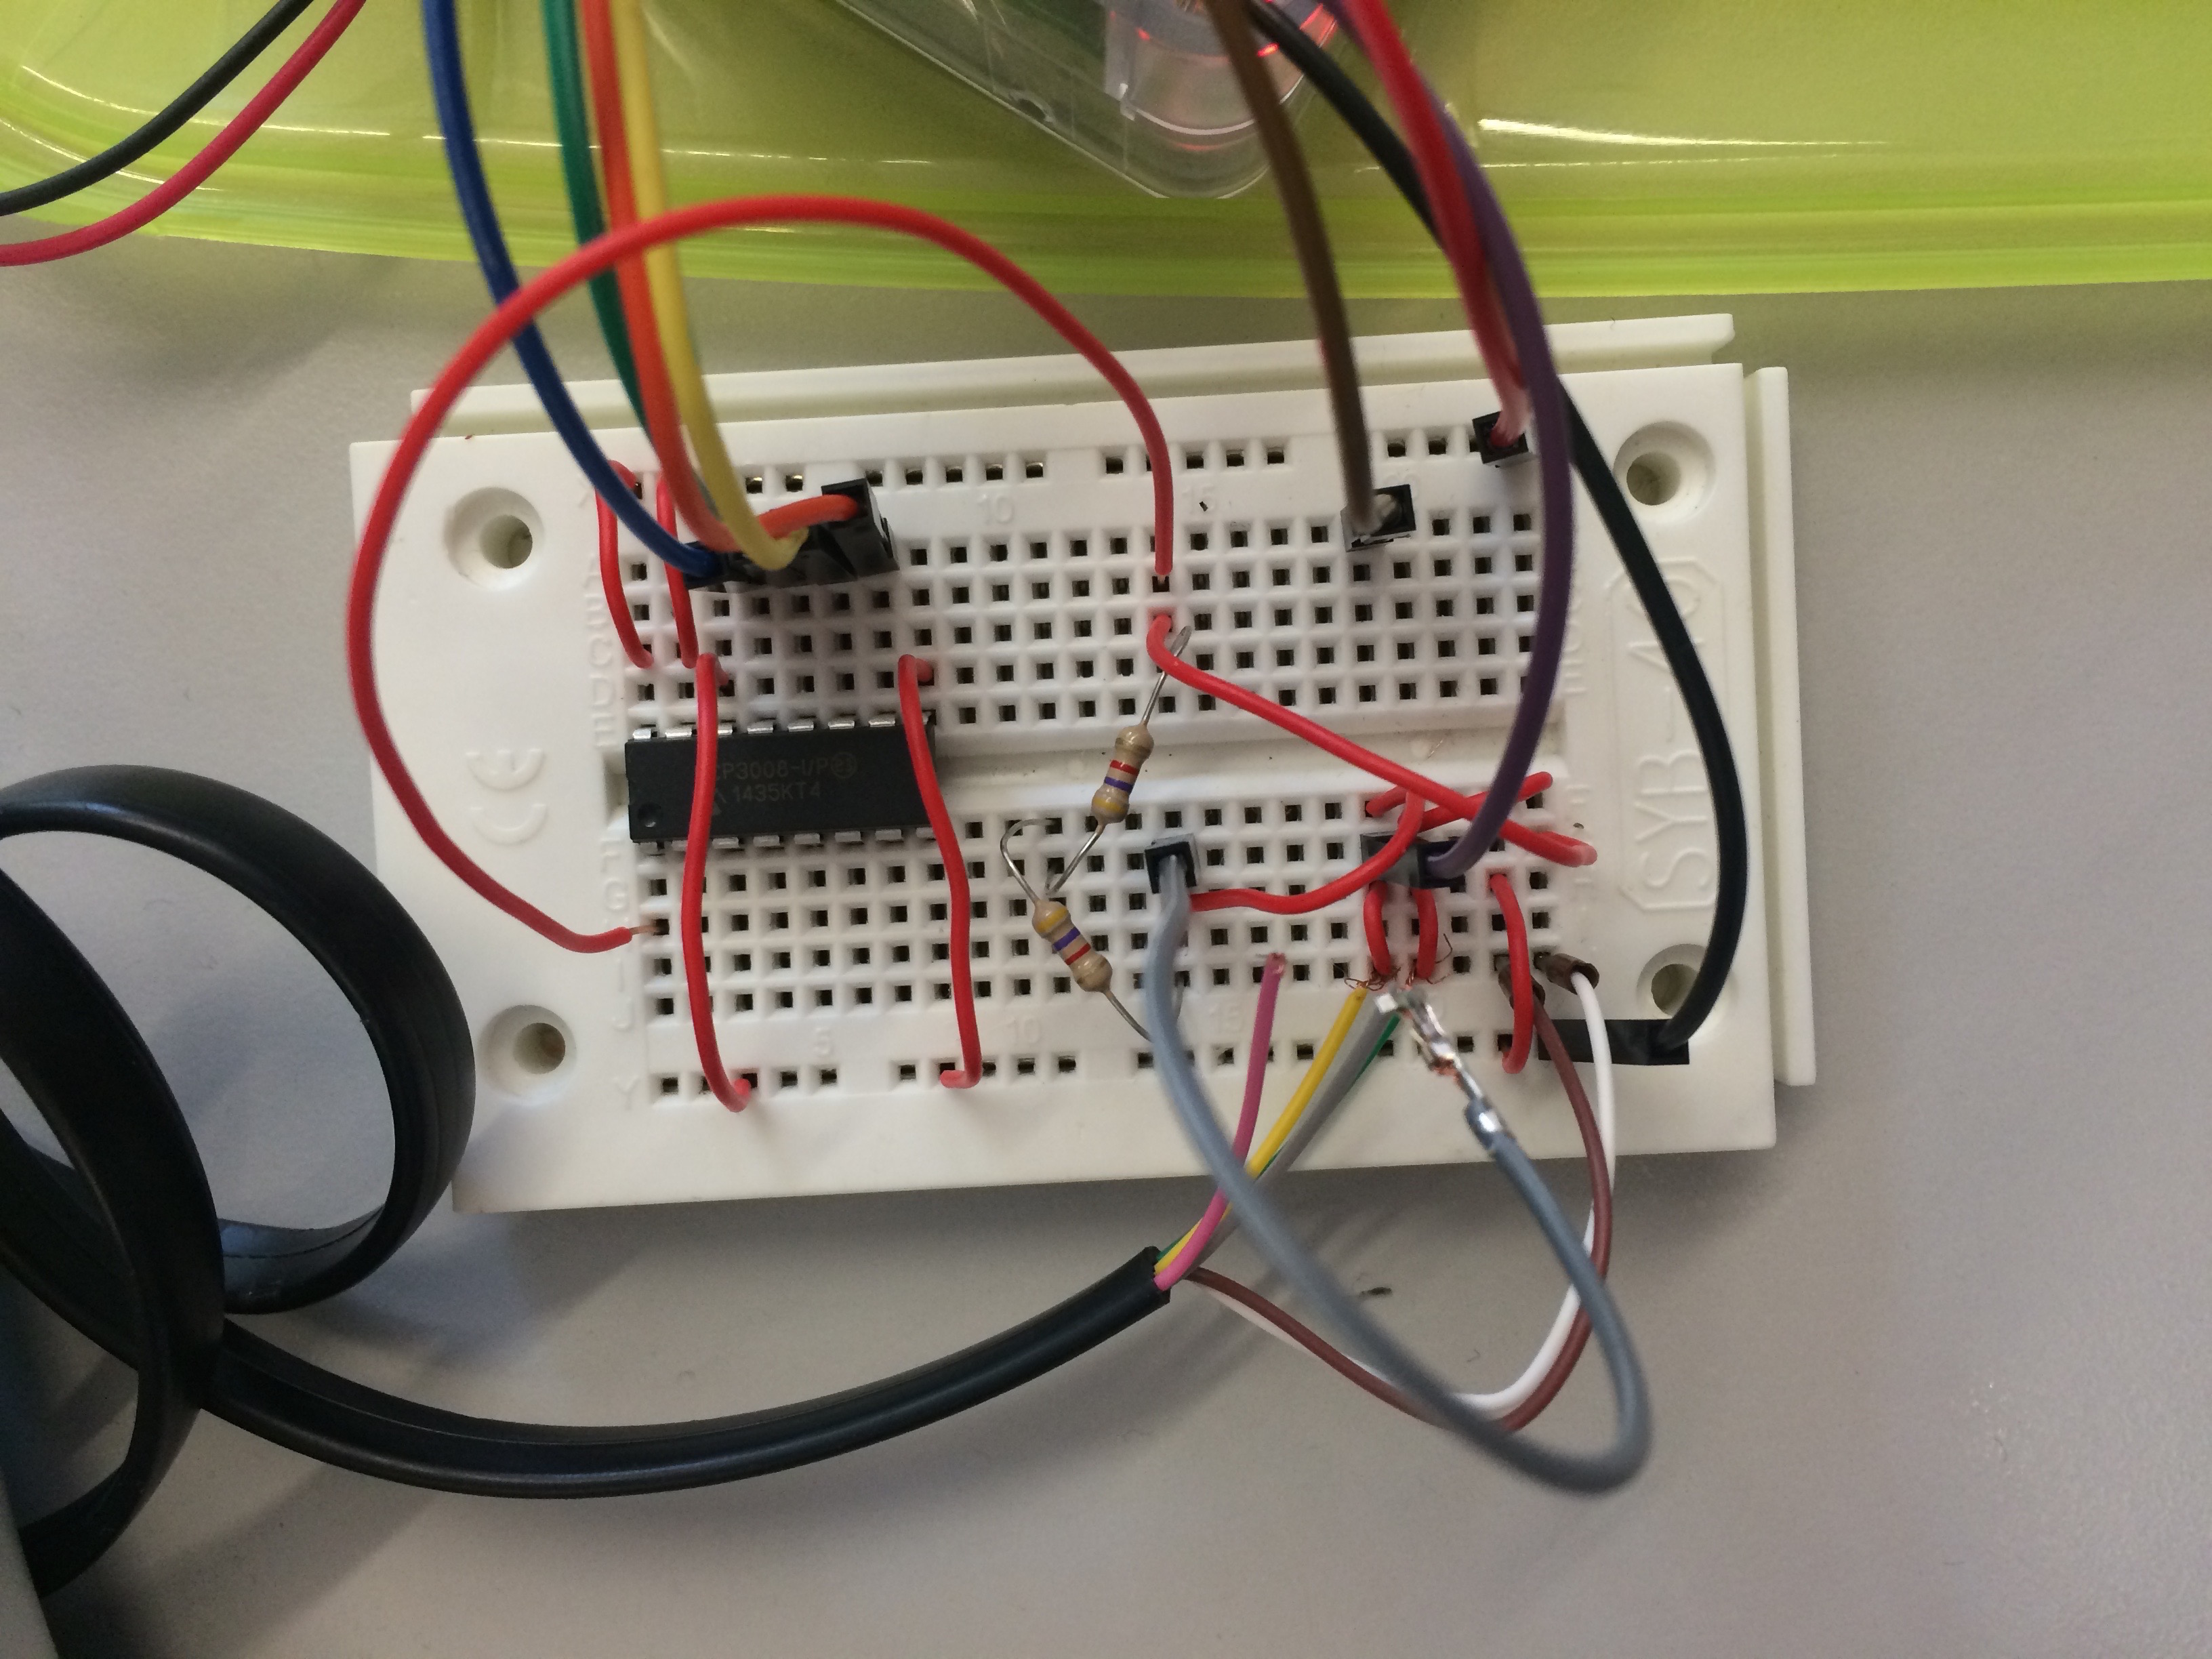
\includegraphics[width=12cm]{schaltung/sensor}
  \caption{Probeaufbau Sensor}
  \label{schaltung:sensor}
\end{figure}

\subsection{Komplett}

Die Herrausforderung die komplette Schaltung zu löten bestand darin die Bauweise so kompakt wir möglich zu gestalten. In der folgenden Liste sind die Bauteile der Schaltung aufgelistet:

\begin{itemize}
  \item 6x female Stecker für NXT Kabel (\EUR{5})
  \item MCP3008 (\EUR{2,5})
  \item SN754410 (\EUR{2,5})
  \item Lochrasterplatine \EUR{1})
  \item 4x 10kOhm Widerstand (\EUR{<1})
  \item 10x female-male Verbindungskabel (<\EUR{1})
  \item Lötzinn und Kupferdraht
\end{itemize}

Die Gesamtkosten der Platine sind mit ca. \EUR{13} sehr gering ausgefallen. Wenn die Kosten eines Raspberry Pi (\EUR{40}) von noch dazugerecht werden, liegen die Gemsamtkosten bei ungefähr \EUR{50}.

Alle Bauelemente lassen sich leicht auf der Lochrasterplatine befestigen. Eine Außnahme stellen die female Stecker da, welche keinen Standartabstand der Pins haben. Hier muss der Kupferdraht direkt angelötet werden.

%Figure
\begin{figure}[h]
  \centering
  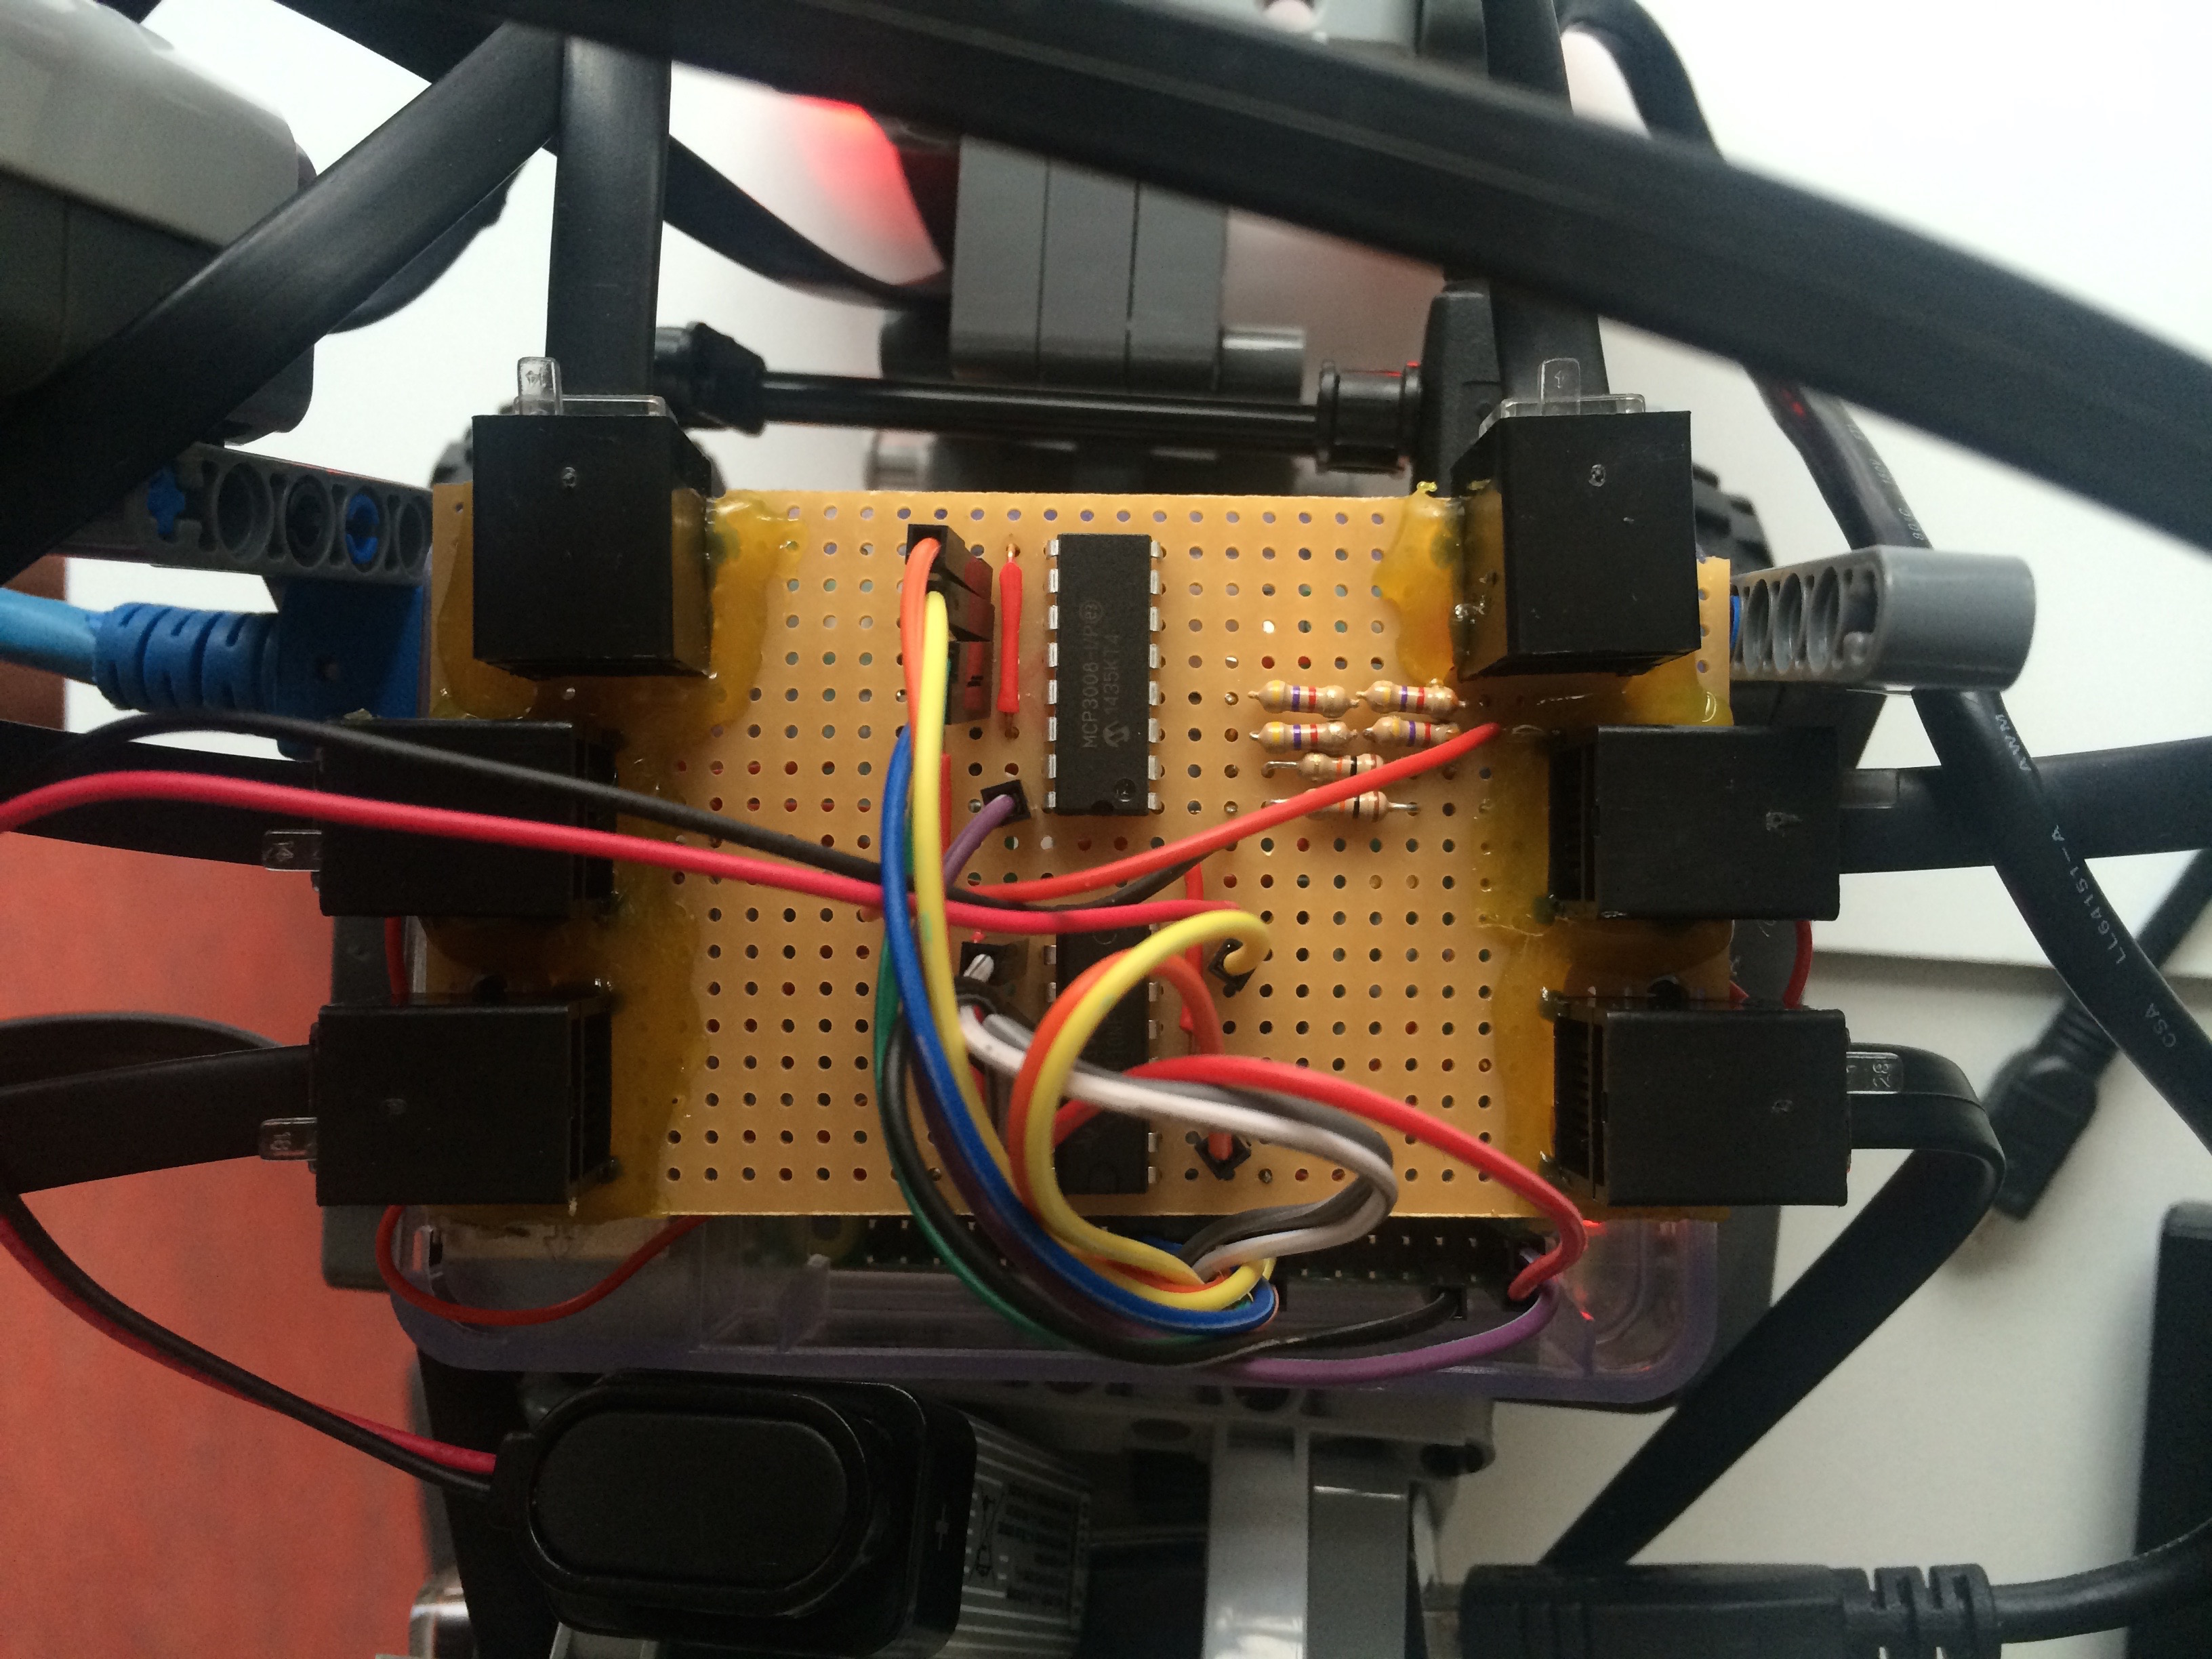
\includegraphics[width=12cm]{schaltung/komplett}
  \caption{Komplette Schaltung}
  \label{schaltung:komplett}
\end{figure}
